\problemname{Tycho}

\illustration{.4}{img/MarsPerseveranceRover.jpg}{}

\noindent
Planetą tyrinėjantis robotas \emph{Tycho VIII} surinko mineralų pavyzdžių ir turi grįžti į bazę.
Tycho keliauja tiesia linija nuo koordinatės~$0$ iki bazės, kurios koordinatė yra~$b$.
Tycho juda lėtu, tačiau pastoviu $1$~ilgio vieneto per sekundę greičiu.
Kas sekundę Tycho patiria $1$~žalos iš aplinkos vienetą dėl atšiaurių planetos sąlygų.

Situacija dar prastesnė dėl radiacijos, sklindančios iš netoliese esančio pulsaro. 
Dėl šios radiacijos robotas papildomai patiria $d$ žalos vienetų kas $p$ sekundžių.
Visgi radiacinės žalos galima išvengti pakeliui pasislėpus vienoje iš $n$ skirtingų slėptuvių 
(uolų, augmenijos, didžiulių akmenų, planetos megafaunos karkasuose griaučiuose).
Tycho bet kurio metu gali pasirinkti ir nejudėti kiek tik nori sekundžių.

Pradinė pozicija, kurios koordinatė yra~$0$, ir bazė, kurios koordinatė yra~$b$, yra apsaugotos,
tad ten Tycho nepatiria radiacinės žalos.

\medskip
Kiek mažiausiai žalos Tycho patirs kelionėje atgal į bazę?

\section*{Pavyzdys}

Paimkime situaciją, kuomet bazės koordinatė yra $18$, o slėptuvės yra koordinatėse $8$ ir $15$.

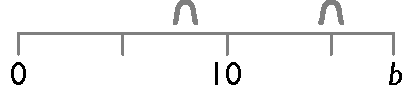
\includegraphics[width=.3\textwidth]{img/samplesetup}

Tarkime, kad pulsaro periodas yra $4$, tad neapsaugotas Tycho patirtų žalos laiko momentais $4$, $8$, $12$, ir t.t.
Jeigu Tycho pajudėtų iš pradinės pozicijos (kur jis yra saugus) laiko momentu $0$, tai galėtų pasiekti pirmąją slėptuvę po $8$ sekundžių, taip patirdamas radiacinės žalos $d$ laiko momentu $4$ (bet ne laiko momentu $8$, kadangi tuo metu jis vėl būtų apsaugotas).
Judėdamas nesustodamas jis pasiektų bazę laiko momentų $18$, patirdamas dar $d+d$ vienetų radiacinės žalos (laiko momentais $12$ and $16$).
Šiuo atveju jis patirtų $d+d+d=3d$ vienetus radiacinės žalos ir
$18$ vienetų žalos iš aplinkos.
Tačiau jeigu Tycho palauktų $2$-ojoje slėptuvėje (kurios koordinatė $15$) vieną sekundę, tai pulsas laiko momentu $16$ nepadarytų jam jokios žalos. Tuomet Tycho pasiektų bazę laiko momentų $19$, iš viso patyręs $2d + 19$ vienetų žalos.
Tai būtų geresnis variantas daugumai $d$ reikšmių.
Šios dvi situacijos pavaizduotos čia:

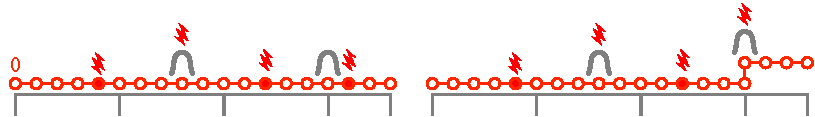
\includegraphics[width=.8\textwidth]{img/sample1_2.pdf}

Jeigu pulsaro periodas yra $10$, Tycho galėtų laukti pradinėje pozicijoje $2$~sekundes ir tuomet judėti į bazę nesustodamas.
Taip Tycho praeitų $1$-ąją slėptuvę (kurios koordinatė yra~$8$) būtent tuo metu, kai pulsaras supulsuotų, ir atvyktų į bazę laiko momentu $20$, iš viso patirdamas $20$ vienetų žalos iš aplinkos ir jokios radiacinės žalos.	

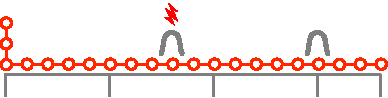
\includegraphics[width=.4\textwidth]{img/sample3.pdf}

\section*{Įvestis}

Pirmoje eilutėje pateikti atskirti tarpais keturi sveikieji skaičiai $b$, $p$, $d$ ir $n$:
bazės koordinatė $b$,
pulsaro pulsavimo periodas~$p$,
papildoma radiacinė žala~$d$, daroma kiekvieno pulsaro pulsavimo metu,
skaičius~$n$, kiek yra slėptuvių.
Kitose $n$~eilučių pateikta po sveikąjį skaičių -- slėptuvių koordinatės $a_1$, $\ldots$, $a_n$, kurioms galioja
$0<a_1<\cdots <a_n< b$. % constraint:shelterbounds, constraint:sortedshelters

\section*{Išvestis}

Išspausdinkite vieną sveikąjį skaičių: mažiausią žalos kiekį, kurį Tycho patirs norėdamas pasiekti bazę ties koordinate $b$.

\section*{Ribojimai ir vertinimas}

Visada galios
$p < b$ % constraint:pulsehappens
ir
$n < b$. % constraint:sheltersfit
Taip pat galios ribojimai
$1\leq b\leq 10^{12}$, % constraint:b
$0\leq d \leq 10^6$ %constraint:d
ir
$0\leq n \leq 10^5$. % constraint:n

Jūsų sprendimas bus testuojamas su keliomis testų grupėmis, kurių kiekviena verta tam tikro skaičiaus taškų.
Kiekviena testų grupė sudaryta iš įvairių testų.
Testų grupės taškai skiriami tik išsprendus visus testus, esančius toje grupėje.
Galutinis rezultatas lygus daugiausiai surinkusio sprendimo taškų skaičiui.

\medskip
\begin{tabular}{lll}
Grupė & Taškai & Ribojimai \\\hline
  $1$ & $8$  & $p\leq 10^6$ ir Tycho nereikės laukti \emph{pajudėjus} iš pozicijos ties koordinate~$0$.$^*$ \\ % constraint:nowait
  $2$ & $5$  & $b\leq 1000$, $p\leq 100$, $n\leq 10$ \\
  $3$ & $7$  & $b\leq 1000$ \\
  $4$ & $15$ & $p\leq 10^6$, $n\leq 1000$\\
  $5$ & $20$ & $p\leq 100$\\
  $6$ & $35$ & $p\leq 10^6$\\
  $7$ & $10$ & \emph{Jokių papildomų ribojimų}
\end{tabular}

\medskip
\noindent $^*$ Testų grupėje~$1$ Tycho gali tekti palaukti ties koordinate~$0$ \emph{prieš} jam pajudant.
Pavyzdžiui, pavyzdinės įvestys $2$, $3$ ir $4$ (\emph{sample inputs $2$, $3$, $4$}) priklauso testų grupei~$1$.
